\section{自干扰的产生和消除过程}
    
    \frame{\sectionpage}
\begin{frame}{\textbf{多径信道与ALC}}
	\begin{columns}[T] % align columns
		\begin{column}<0->{.40\textwidth}
			\begin{figure}[thpb]
				\centering
				\resizebox{1\linewidth}{!}{
					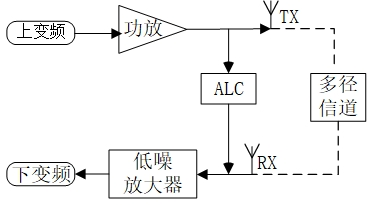
\includegraphics{images/alc.jpg}
				}
				%\includegraphics[scale=1.0]{figurefile}
				$\quad$\caption{多径信道与模拟域线性消除}
				\label{fig:campus}
			\end{figure}
		\end{column}%
		\hfill%
		\begin{column}<0->{.5\textwidth}
			\begin{itemize}
				\item 多径信道中传来的自干扰为$ax_p(t-\delta) + \sum_{c=1}^{L}a_cx_p(t-\delta_c)$
				\item 模拟域线性消除项为$\widehat{a}x_p(t-\widehat{\delta})$
				\item ALC消除结果是
				\begin{equation*}
					\begin{split}
						y_p(t) &= ax_p(t-\delta) - \widehat{a}x_p(t-\widehat{\delta}) \\
						&+ \sum_{c=1}^{L}a_cx_p(t-\delta_c)
					\end{split}
				\end{equation*}
				\item 其中$\forall c\in\{1,\cdots,L\},a_c\sim\mathcal{CN}(0,\sigma^2_{a,c})$
				\item $a\sim \mathcal{CN}(0,\sigma^2_{a})$
			\end{itemize}
		\end{column}%
	\end{columns}
\end{frame}

\begin{frame}
	\begin{block}{$y_p(t)$经过下变频的混频器和低通滤波器后得到}
		\begin{equation*}
			\begin{split}
			\tilde{y}(t) = &\mu_{rx}e^{-j\phi_{rx}(t)} \Big\{  ae^{-j\omega_m\delta}e^{j\phi_{tx}(t-\delta)}[\mu_{tx}x(t-\delta)+\nu_{tx}^{*}x^{*}(t-\delta)] \\
			&- \hat{a} e^{-j\omega_m\hat\delta}e^{j\phi_{tx}(t-\hat\delta)}[\mu_{tx}x(t-\hat\delta)+\nu_{tx}^{*}x^{*}(t-\hat\delta)] \\
			& + \sum_{c=1}^{L}a_ce^{-j\omega_m\delta_c}e^{j\phi_{tx}(t-\delta_c)}[\mu_{tx}x(t-\delta_c)+\nu_{tx}^{*}x^{*}(t-\delta_c)] \Big\}  \\
			&+ \nu_{rx}e^{j\phi_{rx}(t)} \Big\{  a^{*}e^{j\omega_m\delta}e^{-j\phi_{tx}(t-\delta)}[\mu_{tx}^{*}x^{*}(t-\delta)+\nu_{tx}x(t-\delta)] \\
			&- \hat{a}^{*} e^{j\omega_m\hat\delta}e^{-j\phi_{tx}(t-\hat\delta)}[\mu_{tx}^{*}x^{*}(t-\hat\delta)+\nu_{tx}x(t-\hat\delta)] \\
			& + \sum_{c=1}^{L}a_c^{*}e^{j\omega_m\delta_c}e^{-j\phi_{tx}(t-\delta_c)}[\mu_{tx}^{*}x^{*}(t-\delta_c)+\nu_{tx}x(t-\delta_c)]  \Big\}
			\end{split}
		\end{equation*}
	\end{block}
\end{frame}  

\begin{frame}
	\begin{block}{引入$s(t)=x(t-\delta) \approx x(t-\hat\delta),s_c(t)=x(t-\delta_c)$,
			并记$p(t) = e^{j[\phi_{tx}(t-\delta)-\phi_{rx}(t)]} $ 和 $\ p_c(t) = e^{j[\phi_{tx}(t-\delta_c)-\phi_{rx}(t)]}$化简得到}
		\begin{equation*}
		\begin{split}
		\tilde{y}(t)  \approx &\mu_{rx} \Big\{  ap(t)e^{-j\omega_m\delta}[\mu_{tx}s(t)+\nu^{*}_{tx}s^*(t)] \\
		&- \hat{a}p(t)e^{-j\omega_m\hat\delta}[\mu_{tx}s(t)+\nu^{*}_{tx}s^*(t)]  \\
		&+ \sum_{c=1}^{L}a_cp_c(t)e^{-j\omega\delta_c}[\mu_{tx}s_c(t)+\nu^{*}_{tx}s_c^*(t)] \Big\}  \\
		&+ \nu_{rx} \Big\{  a^*p^*(t)e^{j\omega_m\delta}[\mu_{tx}^*s^*(t)+\nu_{tx}s(t)] \\
		&- \hat{a}^*p^*(t)e^{j\omega_m\hat\delta}[\mu_{tx}^*s^*(t)+\nu_{tx}s(t)]  \\
		&+ \sum_{c=1}^{L}a_c^*p^*_c(t)e^{j\omega\delta_c}[\mu_{tx}^*s_c^*(t)+\nu_{tx}s_c(t)] \Big\}
		\end{split}
		\end{equation*}
	\end{block}
\end{frame}

\begin{frame}{抽样和FFT}
	\begin{block}{将$\tilde{y}(t)$经过抽样,再进行FFT}
		\begin{equation*}
			\begin{split}
			y_n &= \mu_{rx} \sum_{c=0}^{L}a_ce^{-j\omega_{m}(cT_s + \delta)+j[\phi_{tx}(nT_s-cT_s-\delta)-\phi_{rx}(nT_s)]} \{ \mu_{tx}s_{n-c}+\nu_{tx}^{*}s^{*}_{n-c} \} \\
			&+ \nu_{rx} \sum_{c=0}^{L}a_c^*e^{j\omega_{m}(cT_s + \delta)-j[\phi_{tx}(nT_s-cT_s-\delta)-\phi_{rx}(nT_s)]} \{ \mu_{tx}^*s^*_{n-c}+\nu_{tx}s_{n-c} \}
			\end{split}
		\end{equation*}
		\begin{equation*}
			\begin{split}
			Y_k &= \sum_{c=0}^{L}a_ce^{-j\omega_{m}(cT_s + \delta)} \big\{ (\mu_{rx}\mu_{tx}S_kW_N^{ck}+\mu_{rx}\nu_{tx}^*S^*_{N-k}W_N^{ck}) \bigotimes P^{(1)}_k  \big\} \\
			&+ \sum_{c=0}^{L}a_c^*e^{j\omega_{m}(cT_s + \delta)}  \big\{ (\nu_{rx}\mu_{tx}^*S^*_{N-k}W_N^{ck}+\nu_{rx}\nu_{tx}S_kW_N^{ck}) \bigotimes P^{(2)}_k  \big\}
			\end{split}
		\end{equation*}
	\end{block}
\end{frame}

\begin{frame}{数字自干扰消除前的自干扰功率是}
	\begin{equation*}
	\begin{split}
	\mathbb{E}|Y[k]|^2 &=\sum_{c=0}^{L}\sigma_{a,c}^2\sum_{l=0}^{N-1}(|\mu_{rx}\mu_{tx}|^2\mathcal{E}_{l}+|\mu_{rx}\nu_{tx}|^2\mathcal{E}_{N-l})\mathbb{E}\big| P^{(1)}[k-l]\big|^2\\
	&+ \sum_{c=0}^{L}\sigma_{a,c}^2\sum_{l=0}^{N-1}(|\nu_{rx}\mu_{tx}|^2\mathcal{E}_{N-l}+|\nu_{rx}\nu_{tx}|^2\mathcal{E}_{l}) \mathbb{E}\big|P^{(2)}[k-l]\big|^2
	\end{split}
	\end{equation*}
	
	其中$\mathbb{E}\big|P^{(i)}[k-l]\big|^2$和收发两端是共用同一个振荡器还是使用两个独立的振荡器有关  
	
\end{frame}

\begin{frame}
	\begin{block}{$\mathbb{E}\big|P^{(i)}[k-l]\big|^2,i=1,2$的理论计算结果}
		\begin{itemize}
			\item 收发两端是共用同一个振荡器\begin{equation*}
			\begin{split}
			\mathbb{E}\big|P^{(i)}[k]\big|^2 =\frac{1}{N^2}\bigg[ -N&+\sum_{n=0}^{c} 2(N-n)e^{-4\pi n\beta T_s}\cos \big(\frac{2\pi kn}{N} \big) \\
			&+e^{-4\pi\beta(cT_s+\delta)}\sum_{n=c+1}^{N-1}2(N-n)\cos\big(\frac{2\pi kn}{N} \big)\bigg].
			\end{split}
			\end{equation*}
			\item 收发两端使用两个独立的振荡器\begin{equation*}
			\mathbb{E}\big|P^{(i)}[k]\big|^2 = \frac{1}{N^2}\bigg[ -N+\sum_{n=0}^{N-1} 2(N-n)e^{-4\pi n\beta T_s}\cos \big(\frac{2\pi kn}{N} \big)\bigg].
			\end{equation*}
		\end{itemize}
	\end{block}
\end{frame}

\begin{frame}{数字域消除后的剩余自干扰功率$\mathbb{E}|U[k]|^2$}
	\begin{columns}[T] % align columns
		\begin{column}<0->{.40\textwidth}
			\begin{equation*}
			\begin{split}
			&\mathbb{E}|U[k]|^2 = \\
			&\sum_{c=0}^{L}\sigma_{a,c}^2\sum_{\substack{l=0 \\ l\neq k}}^{N-1}(|\mu_{rx}\mu_{tx}|^2\mathcal{E}_{l})\mathbb{E}\big| P^{(1)}_{k-l}\big|^2\\
			&+\sum_{c=0}^{L}\sigma_{a,c}^2\sum_{l=0}^{N-1}(|\mu_{rx}\nu_{tx}|^2\mathcal{E}_{N-l})\mathbb{E}\big| P^{(1)}_{k-l}\big|^2\\
			&+ \sum_{c=0}^{L}\sigma_{a,c}^2\sum_{l=0}^{N-1}(|\nu_{rx}\mu_{tx}|^2\mathcal{E}_{N-l}+|\nu_{rx}\nu_{tx}|^2\mathcal{E}_{l}) \mathbb{E}\big|P^{(2)}_{k-l}\big|^2 \\
			&+ |\mu_{rx}\mu_{tx}|^2\mathcal{E}_{k}\mathrm{var}[\widehat{a_c}]\mathbb{E}\big|P^{(1)}_{0}\big|^2.
			\end{split}
			\end{equation*}
		\end{column}%
		\hfill%
		\begin{column}<0->{.4\textwidth}
			它与以下几点有关
			\begin{itemize}
				\item 相位噪声的3-dB带宽;
				\item 多径信道功率;
				\item 模拟域消除和数字域消除水平;
				\item 多径延时;
				\item I/Q不平衡水平.
			\end{itemize}
		\end{column}%
	\end{columns}
\end{frame}
